\chapter{Fuerzas de seguridad y antagonistas}

\begin{figure}[t]
\centering
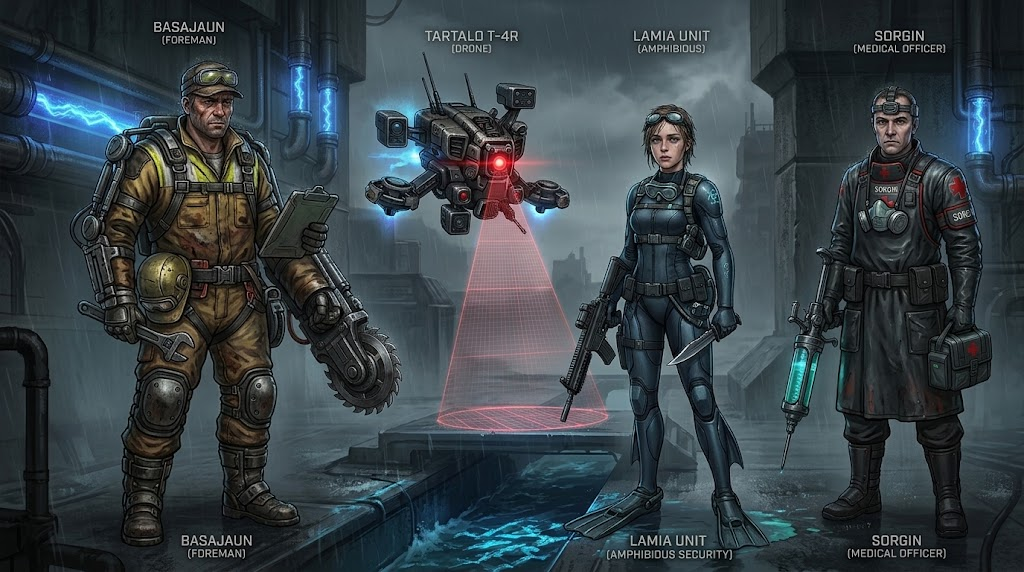
\includegraphics[width=0.95\linewidth]{security_guys.png}
\caption{El archivo corporativo de Ibaizabal-Burdin.}
\end{figure}

\section{Drones Tártalo}

\begin{FichaEnemigo}
\textbf{Nombre:} Tártalo T-4R\par
\textbf{Tipo:} dron de patrulla\par
\textbf{Etiquetas:} \tag{Clandestino}, \tag{Pesado}, \tag{Preciso}, \tag{Vigilado}\par
\textbf{Descripción:} Drones con casco cilíndrico y ojo rojo. Detectan biometría y arritmias. Su luz estroboscópica paraliza por el terror.

\textbf{Amenaza:} los Tártalos son los primeros que detectan a los Fracturados. Empleados en rutas de vigilancia, puntos ciegos y vigilancia industrial.
\end{FichaEnemigo}

\section{Exoesqueletos Basajaun}

\begin{FichaEnemigo}
\textbf{Nombre:} Basajaun\par
\textbf{Tipo:} exoesqueleto industrial\par
\textbf{Etiquetas:} \tag{Contundente}, \tag{Pesado}, \tag{Blindado}\par
\textbf{Descripción:} Capataces y guardias pesados pilotando armaduras de metal, con sierras, ganchos y fuerza de aplastamiento.

\textbf{Amenaza:} avanzan lentamente pero inevitablemente, atravesando pasillos y bloqueando rutas de escape.
\end{FichaEnemigo}

\section{Enjambres Galtzagorri}

\begin{FichaEnemigo}
\textbf{Nombre:} Galtzagorri\par
\textbf{Tipo:} enjambre micro-dron\par
\textbf{Etiquetas:} \tag{Consumible}, \tag{Alta temperatura}, \tag{Desgarrador}\par
\textbf{Descripción:} Pequeños drones al rojo vivo diseñados para reparar grietas y zonas calientes. Sugaar los usa para atacar la respiración y los equipos.

\textbf{Amenaza:} funden armas, cortocircuitan implantes o se cuelan en respiradores para asfixiar a la víctima.
\end{FichaEnemigo}

\section{Unidades Lamia}

\begin{FichaEnemigo}
\textbf{Nombre:} Lamia\par
\textbf{Tipo:} ciborg anfibio\par
\textbf{Etiquetas:} \tag{Oscuro}, \tag{Ácido}, \tag{Aislado}\par
\textbf{Descripción:} Patruyas en canales de enfriamiento y alcantarillas. Emulan voces familiares para desorientar a sus víctimas.

\textbf{Amenaza:} atacan sumergidos, arrastran a la gente bajo el agua ácida y desorientan con sus voces sintéticas.
\end{FichaEnemigo}

\section{División Sorgin}

\begin{FichaEnemigo}
\textbf{Nombre:} Sorgin\par
\textbf{Tipo:} médica de seguridad\par
\textbf{Etiquetas:} \tag{Consumible}, \tag{Clandestino}, \tag{Inyecta}\par
\textbf{Descripción:} Humanas de la casta media con trajes blancos y visores negros, a cargo de la administración incruenta del horror.

\textbf{Amenaza:} no usan armas de fuego. Emplean inyectores de neurotoxinas, drogas de obediencia y amnésicos para mantener el control.
\end{FichaEnemigo}

\section{Resumen táctico}

Los enemigos de NeoBilbao no son solo fuerza bruta. Cada uno tiene un papel distinto dentro del diseño del terror:
\begin{itemize}
  \item Los Tártalos vigilan.
  \item Los Basajaun aplastan.
  \item Los Galtzagorri abrasan.
  \item Las Lamiak arrastran.
  \item Las Sorgin administran el dolor, la obediencia y la narración del miedo.
\end{itemize}

Cada amenaza functiona como una extensión del mismo sistema: la Cúpula no necesita destruir a la gente. Solo necesita mantenerla asustada, rendida y a la vez convencida de que el dolor tiene un sentido.
